% !TEX root =../LibroTipoETSI.tex
\chapter{Denegación de Servicio}\LABCHAP{Denegacion de Servicio}
\pagestyle{esitscCD}
\epigraph{ Denial of Service: ``The prevention of authorized access to resources or the delaying of time critical 
operations''. }{ITU-T recommendation X.800}

% TODO terminar introducción del capítulo
% TODO cambiar todos los TCP, UDP, ICMP, SYN, ACK, DNS por sus acrónimos
%\lettrine[lraise=0.7, lines=1, loversize=-0.25]{E}{l} 
\lettrine[lraise=-0.1, lines=2, loversize=0.25]{E}n este capítulo trataremos de definir qué es un \gls{DoS} 
\index{DoS}, qué significa que un ataque de denegación de servicio sea distribuido \acrshort{DDoS} \index{DDoS}, por 
qué es importante su prevención, por qué es tan difícil su identificación y defensa, esto es, la motivación del 
proyecto.

Las diferentes secciones seguirán la misma clasificación que siguen S.V. Raghavan y E. Dawson en su libro ``An 
Investigation into the Detection and Mitigation of Denial of Service (DoS) Attacks'' \cite{Raghavan}.

%http://en.wikibooks.org/wiki/LaTeX/List_Structures#Customizing_Lists
\section{Definición y consecuencias de un ataque de denegación de servicio} \label{sec:Tipos de ataques DoS}
La seguridad de la información se puede dividir en tres sectores: confidencialidad, esto es, la 
información sólo es vista por los destinatarios; integridad, esto es, la información no ha sido 
alterada desde que se registró y, por último, disponibilidad: El destinatario puede obtener la 
información siempre que la necesite. Un sistema es seguro en la medida que cumple estas tres 
condiciones.

La definición formal que ofrece la \gls{ITU-T} en su recomendación X.800 es la siguiente \cite{ITU-T_DDoS_def}:

\begin{quote}
 The prevention of authorized access to resources or the delaying of time critical operations.
\end{quote}

Por su parte, el \gls{CNSS} ofrece una definición más general \cite{CCNS_DDoS_def}:

\begin{quote}
 Any action or series of actions that prevents any part of an information system from functioning.
\end{quote}

Así pues, los ataques de denegación de servicio atacan directamente a la disponibilidad. Esta falta de disponibilidad 
pueda ser debida a acciones maliciosas o no, originadas de manera local al sistema que se desea proteger o remotamente.

Para impedir el acceso a los recursos, el atacante puede atacar cualquier eslabón de la cadena: Desde el ancho de banda 
de la red que conecta el usuario con el mismo, la memoria o capacidad de procesamiento de la que dispone el sistema, 
alguna debilidad del protocolo de red o la aplicación usada, o cualquier otro sistema que consiga dicho fin 
\cite{Raghavan}.

De esa forma, la empresa que posee el recurso se queda sin los beneficios que el mismo genera durante un periodo de 
tiempo. 

\section{Divide y vencerás: DoS distribuidos}
La principal clasificación que se puede hacer de los ataques de denegación de servicio es en base al número de 
ordenadores atacantes. Si hay más de uno, entonces estamos hablando de un ataque de denegación de servicio distribuido. 
No se debe confundir con los tipos \emph{Spoofing}\footnote{Se definirán mejor estos ataques en el 
\SSSEC{DoS por inundacion}}, que consisten realmente en falsear la dirección de origen de 
las PDU usadas en el ataque. Tras ello, todos los ataques que describiremos a continuación pueden ser distribuidos o no 
(aunque, obviamente, los ataques relacionados con la fuerza bruta tienen más sentido distribuirlos que aquellos que no).

No es raro ver que los atacantes son cientos o miles, y se han llegado a registrar ataques con millones de atacantes. 
La mayoría de los atacante son simplemente nodos infectados con algún tipo de virus o gusano informático, controlados 
y sincronizados remotamente. Estos ordenadores, entonces, pasan a denominarse ordenadores zombis o \emph{bots} 
\index{Bot} \index{Zombi}, controlados por un nodo maestro, y pasan a formar parte de la llamada 
\emph{botnet}\index{Botnet}.

Se da una descripción más detallada de las botnets en la \SEC{BOTNET}.

\section{Taxonomía de un ataque de denegación de servicio}
Las definiciones dadas hasta ahora de ataque de denegación de servicio han sido bastante amplias: Hemos acotado qué 
queremos defender, pero no cómo pueden atacarlo, ni qué parte del sistema de comunicación atacarán. Y esto es necesario 
si queremos definir un sistema de defensa efectivo.

A modo de simplificación, en este trabajo asignaremos a los ataques de denegación de servicio dos características 
diferenciadoras: Sistema de ataque, y objetivo del ataque. De esta forma, podremos entender el por qué del diseño del 
sistema de defensa escogido.

\subsection{Sistema de ataque}
\subsubsection{DoS por inundación}\LABSSSEC{DoS por inundacion}\index{Ataques por inundación} \index{Flooding attacks}
Bajo esta categoría clasificaremos aquellos ataques dirigidos a agotar los recursos que realizan alguna función 
directamente relacionada con ofrecer el servicio. Principalmente, los recursos objetivos suelen ser la memoria, la CPU 
y el ancho de banda, aunque también pueden ir dirigidos a agotar, por ejemplo, el espacio de almacenamiento disponible. 
De esa forma, no queda ningún recurso para que un usuario legítimo pueda hacer uso de ellos.

Este tipo de ataque necesita que el atacante tenga suficientes recursos como para limitar los del atacado. Normalmente, 
un solo atacante no tendrá recursos suficientes para saturar, por ejemplo, un servicio expuesto a Internet. Es ahí 
donde resalta la utilidad de usar un ataque distribuido: Muchísimos atacantes pequeños son capaces de tumbar un 
servicio preparado para atender muchos clientes.

Actualmente, se ofrecen en Internet muchísimos servicios de botnets, haciendo que llevar a cabo un ataque de fuerza 
bruta por inundación sea fácilmente realizable.

Un ejemplo clásico de este tipo de ataque es la inundación de paquetes SYN TCP \index{SYN} \index{TCP}. Para que una 
conexión TCP llegue a ser válida, es necesario que el cliente envíe al servidor \index{Servidor} un paquete TCP de 
sincronía (esto es, con la bandera SYN activa), el servidor le responda con un paquete SYN+ACK \index{ACK} (esto es, con 
las dos banderas activas, SYN y ACK) y el cliente \index{Cliente} devuelva un primer ACK.

Si un cliente sólo envía paquetes SYN, el servidor se ve obligado a mantener una serie de conexiones medio abiertas, lo 
cual terminará por agotar los recursos del servidor (la víctima).

\paragraph{Ataques coordinados por seres humanos}\mbox{\newline}

\noindent Si existen muchos atacantes que requieren intervención manual para realizar el ataque, estamos hablando de un 
ataque DDoS coordinado por seres humanos. 

Un ejemplo de este tipo de ataque es el ataque denominado F5 \cite{F5_attack}. En él, un estudiante intentó tirar abajo 
la red de su escuela convenciendo a muchos estudiantes de que se conectasen a una página determinada y, a una hora 
concreta, presionasen al mismo tiempo el botón \emph{F5} (actualizar página en la mayoría de los navegadores) durante 
un periodo de tiempo.

Otro ejemplo de ataques de este tipo suceden con bastante frecuencia en el denominado \emph{efecto slashdot} (o, el 
equivalente español, efecto barrapunto/menéame). Slashdot es un servicio de noticias muy usado en todo el mundo, al 
igual que sus equivalentes españoles meneame y barrapunto, en el que se acumulan enlaces a noticias subidas por los 
propios usuarios, que son votadas y promocionadas.

Cuando una de esas noticias se encuentra alojada en un servidor con pocos recursos, es frecuente que esta quede 
inaccesible por sobrecarga de recursos. Pese a que la intención de los usuarios era legítima, el sitio ha sufrido un 
\gls{DDoS} según las definiciones anteriores.

\paragraph{Ataques amplificados}\mbox{\newline} \index{Ataques amplificados}

\noindent Un ataque amplificado ocurre cuando el atacante es capaz de generar una respuesta automática de muchos nodos 
de la red, dirigidas a la dirección de la víctima. En la \FIG{amplificacion} podemos ver una descripción gráfica de lo 
que ocurre en este ataque.

\begin{figure}[htbp]
\centering
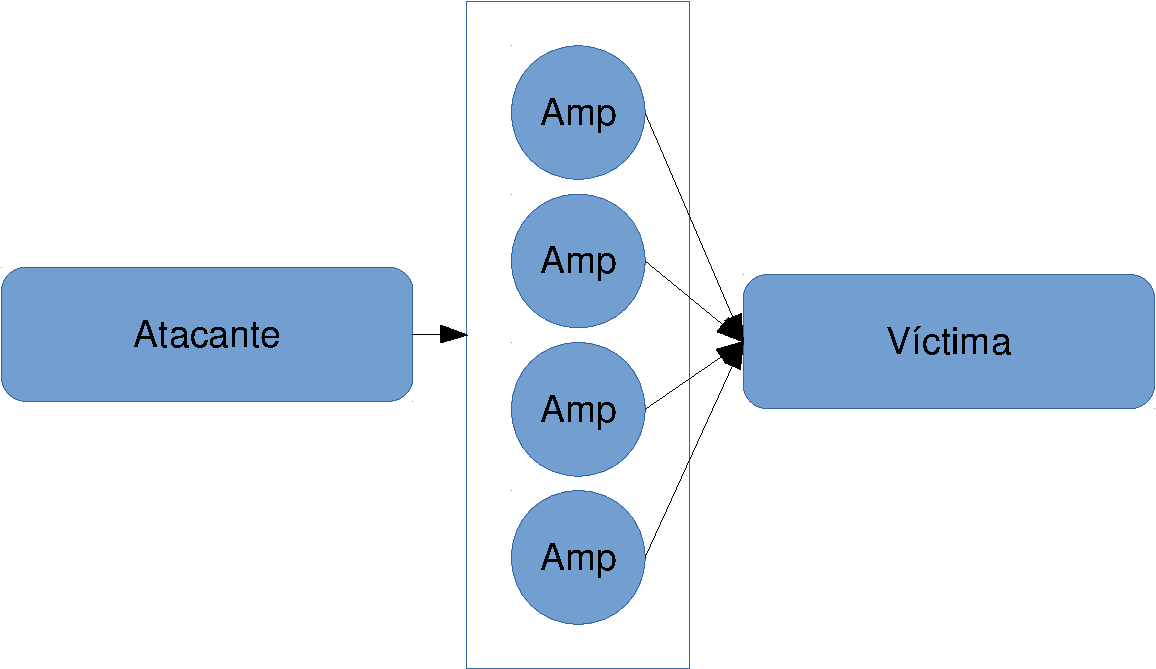
\includegraphics[width=.8\textwidth]{CapituloDDoS/Figuras/Amplificacion}
\caption{Ataque por amplificación}
\LABFIG{amplificacion} %Esto es una forma propia de los autores de gestionar las etiquetas y referencias
\end{figure}
%

Normalmente, este tipo de ataques utilizan la dirección de difusión o broadcast \index{broadcast} \index{difusión}. La 
dirección de difusión es una dirección especial en las redes en las que todos los nodos recibirán el paquete. Si ese 
paquete es una petición que requiere una respuesta, y tiene como dirección origen la dirección IP de la víctima (IP 
spoofing\index{IP Spoofing}), todos los nodos de la red responderán el mensaje, saturando la máquina objetivo.

Un ejemplo sencillo de este tipo de ataque es el denominado Ataque \emph{Smurf} \index{Smurf}, que utiliza un 
simple ICMP\index{ICMP} PING\index{ICMP}\index{PING}. Si a todos los nodos de la red les llega una petición de PING 
proveniente de la dirección de la víctima, la víctima se encontrará con tantas respuestas como nodos configurados para 
responder tenga la red. Dichas respuestas tendrán que ser, al menos, procesadas por el sistema operativo de la máquina 
objetivo, que terminará saturando. Por otro lado, el contenido de la respuesta será una copia del contenido de la 
petición, por lo que es sencillo multiplicar (amplificar) el ancho de banda consumido por la víctima emitiendo un 
paquete grande.

Una variante del anterior es el ataque \emph{Fraggle}. El protocolo UDP\index{UDP} tiene su propio sistema de PING, en 
el puerto 7. Además, tiene un sistema de generación de cadenas aleatorias en el puerto 19, el cual envía cadenas de 
texto aleatorias de longitud aleatoria (pero reducida) cualquiera que las pida. De nuevo, la mecánica del ataque es 
falsear la dirección de origen para que estos servicios respondan a la víctima, saturando así la capacidad de sus 
recursos.

\paragraph{Ataques reflejados}\mbox{\newline} \index{Ataques reflejados}

\noindent Para este apartado, un reflector es un nodo que responde a un paquete con otro paquete destinado a la 
dirección origen del primer paquete. Así, podríamos englobar en este apartado, por ejemplo, servidores DNS\index{DNS}. 
Ver \FIG{reflexion}.

\begin{figure}[htbp]
\centering
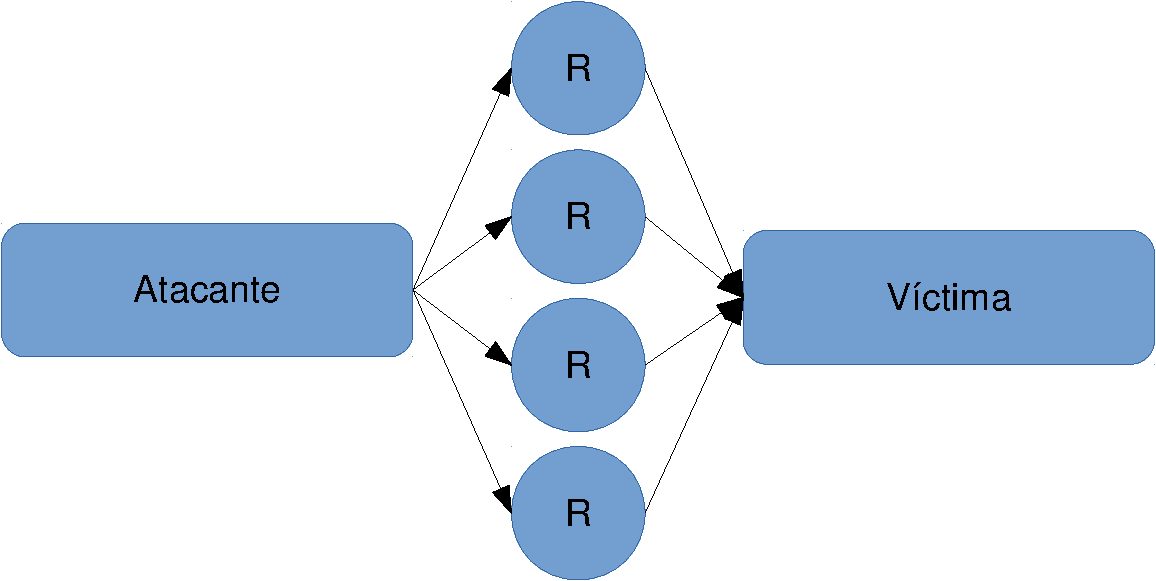
\includegraphics[width=.8\textwidth]{CapituloDDoS/Figuras/Reflexion}
\caption{Ataque por reflexión}
\LABFIG{reflexion} %Esto es una forma propia de los autores de gestionar las etiquetas y referencias
\end{figure}
%

El atacante, entonces, crea una lista de IP reflectoras, y envía para el ataque una petición a cada una de las 
direccionas, con dirección origen la de la vícima. De esta forma, localizar y detener el ataque se vuelve mucho más 
difícil, ya que, siguiendo el ejemplo, cada servidor DNS tiene un dirección IP que no tiene nada que ver con el resto.

Sin embargo, nada impide, en principio, combinar este ataque con el tipo amplificación (por ejemplo, si se 
disponen de muchos DNS en la misma subred). Por otra parte, es posible hacer una petición recursiva a un servidor DNS, 
de forma que en la respuesta viaja el resultado de cada servidor DNS. Esto es, con una pequeña petición (cabecera UDP, 
DNS y nombre de dominio pedido) obtenemos una respuesta mucho mayor, y ya dirigida a la dirección de la victima. 

Así pues, la diferencia entre este tipo y el anterior es que el atacante necesita de una lista de direcciones de host, 
e ir iterando para conseguir el efecto deseado, mientras que en la otra cada paquete se amplificaba mediante el uso de 
la difusión.

\paragraph{Ataques basados en botnets}\mbox{\newline}

\noindent Un bot o zombi es un equipo infectado y controlado remotamente por un maestro. Éste puede ser usado para 
enviar correo no deseado, distribuir malware, espiar (esnifar\index{esnifar tráfico}) tráfico o, en nuestro caso de 
estudio, para perpetrar un ataque de denegación de servicio. 

Gracias a la red de zombis, el atacante real es mucho más difícil de localizar, además de servir como una primera etapa 
de amplificación del ataque.

\subsubsection{DoS Semánticos}
Esta segunda forma de ataque no se basa en la fuerza bruta o en la extenuación de recursos, sino en 
provocar que el servidor\footnote{O algún elemento de la infraestructura de la comunicación} entre en un estado 
\emph{ilegal}, de forma que no pueda ofrecer el servicio. No es necesario un atacante (o varios) con mucha fuerza, sino 
que se puede llevar a cabo con muy pocos recursos. Sin embargo, requiere un conocimiento mucho más profundo del 
servidor y canal de comunicación. Eso sí, el ataque es más sutil y, lo más importante, puede ser corregido con una 
adecuada configuración o actualización de componentes.
 
Uno de los principales ataques de este estilo consiste en enviar información concreta que sabemos de antemano que 
provocará una caída o malfuncionamiento en el servidor, es decir, aprovechando un fallo de seguridad. Por ejemplo, hasta 
hace relativamente poco (1997), el famoso \emph{ping de la muerte} \cite{Bidou} era capaz de tumbar un servidor con tan 
sólo un comando: \texttt{ping <objetivo>\ -l 65511}, el cual viene integrado en todos los sistemas operativos. Éste 
aprovechaba que la pila ICMP asumía que el paquete tenía una longitud determinada. Al procesar el paquete, y superarse 
esta longitud, se producía un desbordamiento de buffer que hacía que el servidor colapsase.

Otro ejemplo de ataque de este tipo es el ataque \emph{land\index{Land attack}}. En él, la victima recibe un paquete 
TCP cuya dirección origen y destino es él mismo, por lo que intenta contactar consigo mismo hasta que colapsa. 

El ataque \emph{\index{teardrop}} también es muy famoso, consistente en enviar mensajes IP fragmentados y malformados a 
la muina objetivo. De esta forma, al intentar des-fragmentarlos, la máquina colapsa.

Las nuevas tecnologías tampoco son inmunes a este tipo de ataque. IPv6, por ejemplo, puede sufrir de \emph{Anuncio de 
vecino envenenado\index{neighbour advertisement spoofing attack}}. En él, un equipo intermedio se anuncia como poseedor 
de una dirección en el camino del cliente al servidor (o bien, la dirección del propio servidor), y anuncia su 
dirección MAC para que todos los paquetes destinados al servidor le lleguen a él. Esto es, es la versión IPv6 del ARP 
spoofing.

\subsection{Objetivo del ataque}

\subsubsection{Ataque a dirigido a redes}
% \subsubsection{Ataque a redes de telefonía móvil} TODO lo meto?
\subsubsection{Ataque a Sistemas Operativos}
\subsubsection{Ataques dirigidos a aplicaciones (Ataques capa 7)}

\section{Arquitectura de una botnet} \LABSEC{BOTNET}
\section{Técnicas de detección de un ataque DDoS}
\section{Técnicas de mitigación de un ataque DDoS}

\section{Resumen}%%%%%%%%%%%%%%%%%%%%%%%%%%%%%%%%%%%%%%%
Para incluir un resumen de una sección o un conjunto de secciones o en cualquier otro punto que consideremos interesante, se utiliza el entorno \comando{begin\{Resumen\}}, que admite como parámetro opcional un nombre que queramos asignarle al resumen. Por defecto, se denomina ``Resumen''. Observar que se ha modificado la cabecera de las páginas impares. Una vez finalizado el resumen, con el comando \comando{end\{Resumen\}}, se recupera la anterior cabecera automáticamente. Los resúmenes que se deseen incluir aparecen en la tabla de contenidos como una sección sin numeración, con el nombre elegido o el nombre por defecto de Resumen. En el siguiente ejemplo hemos utilizado este parámetro opcional de nombre.

\begin{Resumen}[Resumen del capítulo]


\subsection*{S1}

\end{Resumen}

